
\section*{Chapitre 11 - Symétrie axiale}
\addcontentsline{toc}{section}{Chapitre 11 - Symétrie axiale}


\subsection*{I. Symétrie axiale}
\addcontentsline{toc}{subsection}{I. Symétrie axiale}

\begin{Définition}[c]
Deux figures sont symétriques par rapport à une droite si ces figures se superposent par pliage le long de cette droite. Cette droite est l'axe de symétrie.
\end{Définition}

\begin{Exemple}
\begin{minipage}[c]{0.4\textwidth}
\begin{center}
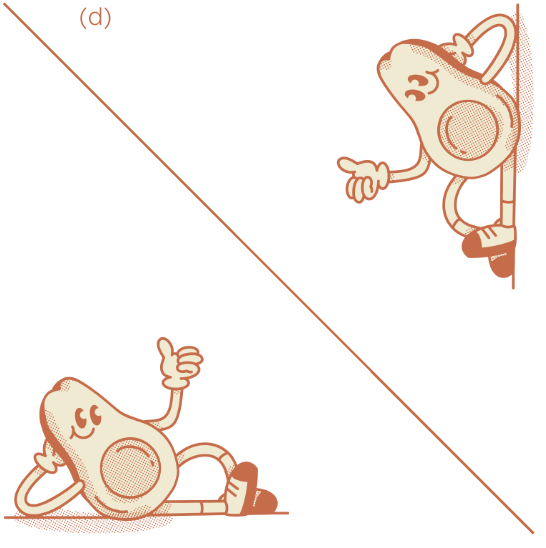
\includegraphics[scale=0.4]{IMG/Avocat} 
\end{center}
\end{minipage} \hfill \begin{minipage}[c]{0.6\textwidth}
\begin{center}
 
\includegraphics[scale=0.6]{IMG/Tacos}
\end{center}
\end{minipage} 

\end{Exemple}



\begin{Propriétés*}
\begin{minipage}[c]{0.7\textwidth}
\begin{itemize}[label=\textcolor{Couleur1}{$\bullet$}]
\item Si un point A n'appartient pas à la droite $(d)$, alors son symétrique par rapport à la droite $(d)$ est le point B tel que $(d)$ est \textbf{la médiatrice du segment [AB]}.
\item Si un point C appartient à la droite $(d)$, alors son symétrique par rapport à la droite $(d)$ est lui-même.
\end{itemize}
\end{minipage}
\begin{minipage}[c]{0.3\textwidth}
\begin{center}
\begin{tikzpicture}[scale=0.8]
\tkzDefPoints{0/0/A, 4/0/B, 2/0/C, 2/2/D, 2/-1.5/E, 2/1.5/F, 2/-0.8/G}
\tkzDrawSegment[line width=0.75](A,B)
\node[below,yshift=-2pt, color=black] at (A) {A};
\node[below,yshift=-2pt, color=black] at (B) {B};
\tkzMarkSegments[mark=|, color=black, pos=0](A,B)
\tkzMarkSegments[mark=|, color=black, pos=1](A,B)
\tkzMarkSegments[mark=s||,color=Couleur1, size=3pt, pos=0.5, thick](A,C C,B)
\tkzDrawSegment[Couleur6](D,E)
\tkzMarkRightAngle[color=Couleur1,size=0.2](D,C,A)
\tkzDrawSegment[dashed, Couleur1](A,F)
\tkzDrawSegment[dashed, Couleur1](B,F)
\node at (2.25,1.75) {C};
\tkzMarkSegments[mark=|, color=black, pos=0](F,C)
\tkzMarkSegments[mark=|, color= Couleur1, pos=0.5,  size=3pt](A,F)
\tkzMarkSegments[mark=|, color= Couleur1, pos=0.5,  size=3pt](B,F)
\end{tikzpicture}
\end{center}
\end{minipage}
\end{Propriétés*}







\begin{Remarque}
Si un point appartient à l'axe de symétrie, alors il est son propre symétrique.
\end{Remarque}

\subsection*{II. Constructions}
\addcontentsline{toc}{subsection}{II. Constructions}

\begin{Exemple}
\begin{enumerate}
\item Construire le triangle  $I'J'K'$ symétrique de $IJK$ par rapport à la droite $(d)$.
\item Coder la figure.

\end{enumerate}

\begin{center}
 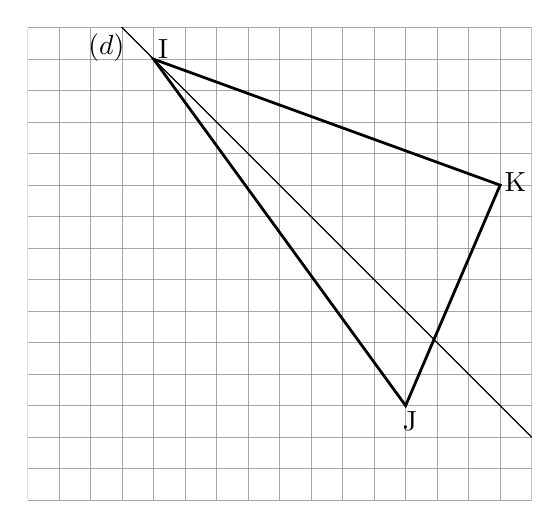
\begin{tikzpicture}[baseline,scale = 0.4]

    \tikzset{
      point/.style={
        thick,
        draw,
        cross out,
        inner sep=0pt,
        minimum width=5pt,
        minimum height=5pt,
      },
    }
    \clip (-8,-10) rectangle (8,5);
    	\draw[color ={gray},opacity = 0.7] (-8,-10)--(-8,5);
	\draw[color ={gray},opacity = 0.7] (-7,-10)--(-7,5);
	\draw[color ={gray},opacity = 0.7] (-6,-10)--(-6,5);
	\draw[color ={gray},opacity = 0.7] (-5,-10)--(-5,5);
	\draw[color ={gray},opacity = 0.7] (-4,-10)--(-4,5);
	\draw[color ={gray},opacity = 0.7] (-3,-10)--(-3,5);
	\draw[color ={gray},opacity = 0.7] (-2,-10)--(-2,5);
	\draw[color ={gray},opacity = 0.7] (-1,-10)--(-1,5);
	\draw[color ={gray},opacity = 0.7] (0,-10)--(0,5);
	\draw[color ={gray},opacity = 0.7] (1,-10)--(1,5);
	\draw[color ={gray},opacity = 0.7] (2,-10)--(2,5);
	\draw[color ={gray},opacity = 0.7] (3,-10)--(3,5);
	\draw[color ={gray},opacity = 0.7] (4,-10)--(4,5);
	\draw[color ={gray},opacity = 0.7] (5,-10)--(5,5);
	\draw[color ={gray},opacity = 0.7] (6,-10)--(6,5);
	\draw[color ={gray},opacity = 0.7] (7,-10)--(7,5);
	\draw[color ={gray},opacity = 0.7] (8,-10)--(8,5);
	\draw[color ={gray},opacity = 0.7] (-8,-10)--(8,-10);
	\draw[color ={gray},opacity = 0.7] (-8,-9)--(8,-9);
	\draw[color ={gray},opacity = 0.7] (-8,-8)--(8,-8);
	\draw[color ={gray},opacity = 0.7] (-8,-7)--(8,-7);
	\draw[color ={gray},opacity = 0.7] (-8,-6)--(8,-6);
	\draw[color ={gray},opacity = 0.7] (-8,-5)--(8,-5);
	\draw[color ={gray},opacity = 0.7] (-8,-4)--(8,-4);
	\draw[color ={gray},opacity = 0.7] (-8,-3)--(8,-3);
	\draw[color ={gray},opacity = 0.7] (-8,-2)--(8,-2);
	\draw[color ={gray},opacity = 0.7] (-8,-1)--(8,-1);
	\draw[color ={gray},opacity = 0.7] (-8,0)--(8,0);
	\draw[color ={gray},opacity = 0.7] (-8,1)--(8,1);
	\draw[color ={gray},opacity = 0.7] (-8,2)--(8,2);
	\draw[color ={gray},opacity = 0.7] (-8,3)--(8,3);
	\draw[color ={gray},opacity = 0.7] (-8,4)--(8,4);
	\draw[color ={gray},opacity = 0.7] (-8,5)--(8,5);
	
	\draw[color={black}] (-35.35533905932737,35.35533905932737)--(36.35533905932737,-36.35533905932737);
	

	\draw [color={black}] (-3.7,4.310352) node[anchor = center, rotate = 0] {I};
	\draw [color={black}] (4.134577,-7.484476) node[anchor = center, rotate = 0] {J};
	\draw [color={black}] (7.486352,0.104218) node[anchor = center, rotate = 0] {K};
	
	\draw[color={black},line width = 1] (-4,4)--(4,-7)--(7,0)--cycle;

	\draw [color={black}] (-5.5,4.353553) node[anchor = center, rotate = 0] {$(d)$};

\end{tikzpicture}
\end{center}
\end{Exemple}
\newpage

\begin{Remarque}
Méthode pour tracer une symétrie axiale à l'aide de l'équerre et du compas : LLS.fr/M6Methode27 \\
Ou à l'aide du compas seulement : https://youtu.be/fjM6sK8NXas?si=xb4Mdj6hnpBmigtC
\end{Remarque}



\begin{Exemple}
\begin{enumerate}
\item Construire le triangle  $M'N'O'$ symétrique de $MNO$ par rapport à la droite $(d)$.
\item Coder la figure.

\end{enumerate}

\begin{center}
 \begin{tikzpicture}[baseline,scale = 0.5]

    \tikzset{
      point/.style={
        thick,
        draw,
        cross out,
        inner sep=0pt,
        minimum width=5pt,
        minimum height=5pt,
      },
    }
    \clip (-7,-9) rectangle (9,7);
    	
	
	\draw[color={black}] (-35.35533905932737,35.35533905932737)--(36.35533905932737,-36.35533905932737);

	\draw [color={black}] (0.922299,6.492109) node[anchor = center , rotate = 0] {M};
	\draw [color={black}] (-0.125392,-8.480671) node[anchor = center , rotate = 0] {N};
	\draw [color={black}] (5.454208,1.20187) node[anchor = center , rotate = 0] {O};

	\draw[color={black}] (1,6)--(0,-8)--(5,1)--cycle;
	
	\draw [color={black}, line width = 1] (-5.646447,6.353553) node[anchor = center, rotate = 0] {$(d)$};

\end{tikzpicture}
\end{center}
\end{Exemple}

\subsection*{III. Propriétés de la symétrie axiale}
\addcontentsline{toc}{subsection}{III. Propriétés de la symétrie axiale}


\begin{Propriétés}[c]
Soit A, B et C trois points ayant respectivement pour symétriques par rapport à une droite $(d)$ les points A', B' et C'.

\begin{enumerate}
\item Le symétrique du segment [AB] est le segment [A'B'] et AB = A'B'.
\item Le symétrique de l'angle $\widehat{ABC}$ est l'angle $\widehat{A'B'C'}$ et $\widehat{ABC} = \widehat{A'B'C'}$.
\item Si A, B et C sont alignés, alors A', B' et C' sont aussi alignés dans le même ordre.
\item Le symétrique d'un cercle de centre A est le cercle de centre A' et de même rayon.
\end{enumerate}
\begin{multicols}{4}
\begin{center}
\begin{tikzpicture}[scale=0.7]
\node at (-5,5.5) {1.};
% Définition des coordonnées des points
\coordinate (A) at (-3,4);
\coordinate (B) at (-4,2);
\coordinate (A') at (-1.6,3.65);
\coordinate (B') at (-1.65,1.4);
\coordinate (C) at (-2,5);
\coordinate (D) at (-3,1);

% Lignes depuis A
\draw[ultra thick, Couleur11] (A) -- (B);
\draw[ultra thick, Couleur11!75] (A') -- (B');
\draw[ultra thick, Couleur1] (C) -- (D);




% Marques d'égalité des segments

% Pour Milieu de AB (un trait perpendiculaire sur chaque segment)
\coordinate (MidAB) at ($(A)!0.5!(B)$);

\draw[thick, gray] ($(MidAB)!0.15cm!90:(B)$) -- ($(MidAB)!0.15cm!-90:(B)$);

\coordinate (MidA'B') at ($(A')!0.5!(B')$);

\draw[thick, gray] ($(MidA'B')!0.15cm!90:(B')$) -- ($(MidA'B')!0.15cm!-90:(B')$);


% Points (croix)
\draw[thick, black] (A) +(-2pt,-2pt) -- +(2pt,2pt);
\draw[thick, black] (A) +(-2pt,2pt) -- +(2pt,-2pt);
\draw[thick, black] (B) +(-2pt,-2pt) -- +(2pt,2pt);
\draw[thick, black] (B) +(-2pt,2pt) -- +(2pt,-2pt);
\draw[thick, black] (A') +(-2pt,-2pt) -- +(2pt,2pt);
\draw[thick, black] (A') +(-2pt,2pt) -- +(2pt,-2pt);
\draw[thick, black] (B') +(-2pt,-2pt) -- +(2pt,2pt);
\draw[thick, black] (B') +(-2pt,2pt) -- +(2pt,-2pt);


% Étiquettes des points
\node[above left] at (A) {A};
\node[below left] at (B) {B};
\node[above right] at (A') {A'};
\node[below right] at (B') {B'};
\node[right] at (D) {$(d)$};


\end{tikzpicture}
\end{center}



\begin{center}
\begin{tikzpicture}[scale=0.8]
\node at (-5,5.5) {2.};
% Définition des coordonnées des points
\coordinate (A) at (-3,4);
\coordinate (B) at (-4,3);
\coordinate (C) at (-4,4.66);
\coordinate (A') at (-1.6,3.65);
\coordinate (B') at (-1.18,2.29);
\coordinate (C') at (-0.4,3.76);
\coordinate (E) at (-2,5);
\coordinate (D) at (-3,1);

% Lignes depuis A
\draw[ultra thick, Couleur8] (A) -- (B);
\draw[ultra thick, Couleur8] (B) -- (C);
\draw[ultra thick, Couleur8!75] (A') -- (B');
\draw[ultra thick, Couleur8!75] (B') -- (C');
\draw[ultra thick, Couleur1] (E) -- (D);






% Points (croix)
\draw[thick, black] (A) +(-2pt,-2pt) -- +(2pt,2pt);
\draw[thick, black] (A) +(-2pt,2pt) -- +(2pt,-2pt);
\draw[thick, black] (B) +(-2pt,-2pt) -- +(2pt,2pt);
\draw[thick, black] (B) +(-2pt,2pt) -- +(2pt,-2pt);
\draw[thick, black] (A') +(-2pt,-2pt) -- +(2pt,2pt);
\draw[thick, black] (A') +(-2pt,2pt) -- +(2pt,-2pt);
\draw[thick, black] (B') +(-2pt,-2pt) -- +(2pt,2pt);
\draw[thick, black] (B') +(-2pt,2pt) -- +(2pt,-2pt);
\draw[thick, black] (C) +(-2pt,-2pt) -- +(2pt,2pt);
\draw[thick, black] (C) +(-2pt,2pt) -- +(2pt,-2pt);
\draw[thick, black] (C') +(-2pt,-2pt) -- +(2pt,2pt);
\draw[thick, black] (C') +(-2pt,2pt) -- +(2pt,-2pt);

% Étiquettes des points
\node[above right] at (A) {A};
\node[below ] at (B) {B};
\node[above ] at (A') {A'};
\node[below ] at (B') {B'};
\node[above ] at (C) {C};
\node[above ] at (C') {C'};
\node[right] at (D) {$(d)$};

% Tracer les angles ABC et A'B'C'
% Angle ABC (angle au point B)
\draw[Couleur8, thick] let \p1 = (A), \p2 = (B), \p3 = (C) in
    (\p2) +({atan2(\y1-\y2,\x1-\x2)}:0.5) arc ({atan2(\y1-\y2,\x1-\x2)}:{atan2(\y3-\y2,\x3-\x2)}:0.5);

% Angle A'B'C' (angle au point B')
\draw[Couleur8!75, thick] let \p1 = (A'), \p2 = (B'), \p3 = (C') in
    (\p2) +({atan2(\y1-\y2,\x1-\x2)}:0.5) arc ({atan2(\y1-\y2,\x1-\x2)}:{atan2(\y3-\y2,\x3-\x2)}:0.5);

% Étiquettes des angles (optionnel)
\node[Couleur8] at (-3.6,4) {\small $45$°};
\node[Couleur8!75] at (-1,3.2) {\small $45$°};
\end{tikzpicture}
\end{center}



\begin{center}
\begin{tikzpicture}[scale=0.7]
\node at (-5,5.5) {3.};
% Définition des coordonnées des points
\coordinate (A) at (-3,4);
\coordinate (C) at (-4,2);
\coordinate (B) at (-3.26,3.48);
\coordinate (A') at (-1.6,3.65);
\coordinate (C') at (-1.65,1.4);
\coordinate (B') at (-1.6,3.07);
\coordinate (E) at (-2,5);
\coordinate (D) at (-3,1);

% Lignes depuis A
\draw[ultra thick, Couleur7] (A) -- (C);
\draw[ultra thick, Couleur7!75] (A') -- (C');
\draw[ultra thick, Couleur1] (E) -- (D);






% Points (croix)
\draw[thick, black] (A) +(-2pt,-2pt) -- +(2pt,2pt);
\draw[thick, black] (A) +(-2pt,2pt) -- +(2pt,-2pt);
\draw[thick, black] (B) +(-2pt,-2pt) -- +(2pt,2pt);
\draw[thick, black] (B) +(-2pt,2pt) -- +(2pt,-2pt);
\draw[thick, black] (A') +(-2pt,-2pt) -- +(2pt,2pt);
\draw[thick, black] (A') +(-2pt,2pt) -- +(2pt,-2pt);
\draw[thick, black] (B') +(-2pt,-2pt) -- +(2pt,2pt);
\draw[thick, black] (B') +(-2pt,2pt) -- +(2pt,-2pt);
\draw[thick, black] (C) +(-2pt,-2pt) -- +(2pt,2pt);
\draw[thick, black] (C) +(-2pt,2pt) -- +(2pt,-2pt);
\draw[thick, black] (C') +(-2pt,-2pt) -- +(2pt,2pt);
\draw[thick, black] (C') +(-2pt,2pt) -- +(2pt,-2pt);

% Étiquettes des points
\node[above left] at (A) {A};
\node[ left] at (B) {B};
\node[above right] at (A') {A'};
\node[ right] at (B') {B'};
\node[below left] at (C) {C};
\node[below right] at (C') {C'};
\node[right] at (D) {$(d)$};


\end{tikzpicture}
\end{center}

\begin{center}
\begin{tikzpicture}[scale=0.7]
\node at (-5,5.5) {4.};
% Définition des coordonnées des points
\coordinate (A) at (-4,4);
\coordinate (B) at (-5,4);

\coordinate (A') at (-0.71,3.18);
\coordinate (B') at (0.18,2.71);

\coordinate (E) at (-2,5);
\coordinate (D) at (-3,1);

% Lignes depuis A
\draw[ultra thick, Couleur6] (A) -- (B);
\draw[ultra thick, Couleur6!75] (A') -- (B');
\draw[ultra thick, Couleur1] (E) -- (D);


\draw[ultra thick,Couleur6] let \p1 = (A), \p2 = (B) in 
    (A) circle ({veclen(\x2-\x1,\y2-\y1)});

\draw[ultra thick,Couleur6!75] let \p1 = (A'), \p2 = (B') in 
    (A') circle ({veclen(\x2-\x1,\y2-\y1)});

% Pour Milieu de AB (un trait perpendiculaire sur chaque segment)
\coordinate (MidAB) at ($(A)!0.5!(B)$);

\draw[thick, gray] ($(MidAB)!0.15cm!90:(B)$) -- ($(MidAB)!0.15cm!-90:(B)$);

\coordinate (MidA'B') at ($(A')!0.5!(B')$);

\draw[thick, gray] ($(MidA'B')!0.15cm!90:(B')$) -- ($(MidA'B')!0.15cm!-90:(B')$);

% Points (croix)
\draw[thick, black] (A) +(-2pt,-2pt) -- +(2pt,2pt);
\draw[thick, black] (A) +(-2pt,2pt) -- +(2pt,-2pt);
\draw[thick, black] (B) +(-2pt,-2pt) -- +(2pt,2pt);
\draw[thick, black] (B) +(-2pt,2pt) -- +(2pt,-2pt);
\draw[thick, black] (A') +(-2pt,-2pt) -- +(2pt,2pt);
\draw[thick, black] (A') +(-2pt,2pt) -- +(2pt,-2pt);
\draw[thick, black] (B') +(-2pt,-2pt) -- +(2pt,2pt);
\draw[thick, black] (B') +(-2pt,2pt) -- +(2pt,-2pt);


% Étiquettes des points
\node[above right] at (A) {A};

\node[above left] at (A') {A'};

\node[right] at (D) {$(d)$};


\end{tikzpicture}
\end{center}
\end{multicols}
On dit que la symétrie axiale \textbf{conserve l'alignement, les mesures de longueurs et d'angles}.
\end{Propriétés}



\newpage

\begin{Exemple}
 Les points $J'$, $V'$, $N'$ sont les images respectives de $J$, $V$, $N$ par la symétrie d'axe $(d)$.\\Compléter l'image du triangle $JVN$ par la symétrie d'axe $(d)$ en utilisant les propriétés de conservation de la symétrie axiale et en justifiant ses démarches.\\
 \begin{minipage}[c]{0.5\textwidth}
 \vspace*{0.3cm}
 
\ligne

\ligne

\ligne

\ligne

\ligne

\ligne

\ligne

\ligne
 \end{minipage} \hfill  \begin{minipage}[c]{0.5\textwidth}
 \begin{center}
 \begin{tikzpicture}[baseline,scale=0.4,transform shape]

    \tikzset{
      point/.style={
        thick,
        draw,
        cross out,
        inner sep=0pt,
        minimum width=5pt,
        minimum height=5pt,
      },
    }
    \clip (-10.771479568461846,-2) rectangle (8.201678919464253,11.190601214735342);
    	\draw[opacity=1] (-6.01698031450355,7.021576775900772) node[anchor = center, rotate=0] {$\ldots^\circ$};
\draw[opacity=1] (-8.5,6.0979734148237865) node[anchor = center, rotate=0] {$\ldots\text{ cm}$};
	\draw[color={black}] (-5.000510804235184,6.706656115005452) arc (-110.38:-200.57999999999998:1) ;
	\draw[color={black}] (-22.847117901547588,-46.229939429384345)--(17.237117901547588,51.05993942938434);
	\draw[color ={black}] (0,0)--(2.19,4.83);
	\draw[color ={black}] (6.2,3.02)--(2.19,4.83);
	\draw[color ={black}] (0,0)--(6.2,3.02);
	\draw [color={black}] (3.320025,1.062983) node[anchor = center , rotate = -334.02944] {6,9 cm};
	\draw [color={black}] (4.399611,4.382167) node[anchor = center , rotate = -24.29306] {4,4 cm};
	\draw [color={black}] (0.638523,2.620074) node[anchor = center , rotate = 65.60969] {5,3 cm};
	\draw [color={black}] (-0.364842,-0.34147) node[anchor = center , rotate = 0] {J};
	\draw [color={black}] (6.698687,3.084223) node[anchor = center , rotate = 0] {V};
	\draw [color={black}] (2.055703,5.307219) node[anchor = center , rotate = 0] {N};
	\draw[opacity=1] (4.701868105751285,3.0009381701468287) node[anchor = center, rotate=0] { \color{black}$50^\circ$};
	\draw[color={black}] (5.302884873165086,2.5863897660555573) arc (-154:-204.18:1) ;
	\draw[opacity=1] (1.0455599515969627,1.0755484124931605) node[anchor = center, rotate=0] {\color{black}$40^\circ$};
	\draw[color={black}] (0.898794046299167,0.4383711467890775) arc (26:65.62:1) ;
	\draw[opacity=1] (2.718539487967943,3.4243517749448533) node[anchor = center, rotate=0] { \color{black}$90^\circ$};
	\draw[color={black}] (1.7750608468454518,3.916523840090381) arc (-114.38:-24.179999999999993:1) ;
	\draw[color={black}] (-6.498096,2.67587)--(-8.77148,9.190601)--(-4.652235,7.644048)--cycle;
	\draw [color={black}] (-6.479504,2.176504) node[anchor = center , rotate = 0] {J'};
	\draw [color={black}] (-9.082496,9.582802) node[anchor = center , rotate = 0] {V'};
	\draw [color={black}] (-4.220479,7.891706) node[anchor = center , rotate = 0] {N'};

\end{tikzpicture}
 \end{center}
  \end{minipage}

\end{Exemple}


\subsection*{IV. Axe de symétrie}
\addcontentsline{toc}{subsection}{IV. Axe de symétrie}

\begin{Définition}
Une figure possède un axe de symétrie si elle est son propre symétrique par rapport à cet axe.
\end{Définition}


\begin{Exemples} Axes de symétrie des figures usuelles
\begin{center}
  \begin{tikzpicture}[scale=0.7, transform shape]
    % Triangle isocèle
    \coordinate (A) at (1.5,2.5);
    \coordinate (B) at (0.5,0);
    \coordinate (C) at (2.5,0);
    \coordinate (D) at (1.5,-0.5);
    \coordinate (E) at (1.5,2.5);
    \coordinate (F) at (1.5,0);
    \draw[line width=1pt,style=dashed, Couleur8] (E) -- (D);
    \tkzMarkSegments[mark=||, color=Couleur8, pos=0.25](B,C)
    \tkzMarkSegments[mark=||, color=Couleur8, pos=0.75](B,C)
    \tkzMarkSegments[mark=|, color=gray, pos=0.5](A,C)
    \tkzMarkSegments[mark=|, color=gray, pos=0.5](B,A)

    % Tracer un arc pour l'angle aigu ABC
    \pic [draw, angle radius=4mm, color=Couleur7, fill=Couleur7!15] {angle = C--B--A};


    % Tracer un arc pour l'angle aigu IJK
    \pic [draw, angle radius=4mm, color=Couleur7, fill=Couleur7!15] {angle = A--C--B};


    % Tracer un angle droit
    \tkzMarkRightAngle[size=0.2, Couleur8](A,F,C)
        \node at (1.5,3.2) {\textbf{Triangle isocèle}};

    \draw[line width=1pt,gray] (A) -- (B) -- (C) -- cycle;
    \end{tikzpicture}
 \hspace*{0.1cm}
   \begin{tikzpicture}[scale=0.7, transform shape] % Triangle équilatéral
    \coordinate (A) at (1.5,2.6);
    \coordinate (B) at (0,0);
    \coordinate (C) at (3,0);
    \coordinate (D) at (1.5,-0.5);
    \coordinate (E) at (1.5,2.8);
    \coordinate (F) at (1.5,0);
    \coordinate (G) at (0,1.73);
    \coordinate (H) at (3.58,-0.33);
    \coordinate (I) at (3.23,1.86);
    \coordinate (J) at (-0.57,-0.33);
    \coordinate (K) at (0.75,1.3);
    \coordinate (L) at (2.25,1.3);
    \draw[line width=1pt,style=dashed, Couleur8] (E) -- (D);
    \draw[line width=1pt,style=dashed, Couleur8] (G) -- (H);
    \draw[line width=1pt,style=dashed, Couleur8] (I) -- (J);
    \tkzMarkSegments[mark=||, color=Couleur8, pos=0.25](B,C C,B A,B B,A A,C C,A)

    % Tracer un arc pour l'angle aigu ABC
    \pic [draw, angle radius=4mm, color=Couleur7, fill=Couleur7!15] {angle = C--B--A};

    % Tracer un arc pour l'angle aigu IJK
    \pic [draw, angle radius=4mm, color=Couleur7, fill=Couleur7!15] {angle = A--C--B};


    % Tracer un arc pour l'angle aigu ABC
    \pic [draw, angle radius=4mm, color=Couleur7, fill=Couleur7!15] {angle = B--A--C};


    % Tracer un angle droit
    \tkzMarkRightAngle[size=0.2, Couleur8](A,F,C)
    \tkzMarkRightAngle[size=0.2, Couleur8](B,K,C)
    \tkzMarkRightAngle[size=0.2, Couleur8](C,L,B)
        \node at (1.5,3.2) {\textbf{Triangle équilatéral}};
    

    \draw[line width=1pt,gray] (A) -- (B) -- (C) -- cycle;
    \end{tikzpicture}
 \hspace*{0.1cm}
    \begin{tikzpicture}[scale=0.7, transform shape]
    % Rectangle
        \tkzDefPoint(0,0){C}
        \tkzDefPoint(3,0){N}
        \tkzDefPoint(3,2){H}
        \tkzDefPoint(0,2){E}
        \tkzDefPoint(1.5,0){M}
        \tkzDefPoint(3,1){P}
        \tkzDefPoint(1.5,2){O}
        \tkzDefPoint(0,1){Q}
        \tkzDefPoint(1.5,1){S}
        \tkzDrawSegments[line width=1pt,gray](C,N N,H H,E E,C)
        \tkzDrawSegments[style=Couleur8, dashed](C,H E,N)
        \tkzLabelSegment[below=2pt](C,N){}
        \node at (1.5,2.6) {\textbf{Rectangle}};
        \draw[line width=1pt,style=dashed, Couleur8] (1.5,-0.5) -- (1.5,2.5);
        \draw[line width=1pt,style=dashed, Couleur8] (-0.3,1) -- (3.3,1);
        \tkzMarkSegments[mark=|, color=Couleur8, pos=0.25](C,N N,C H,E E,H)
        \tkzMarkSegments[mark=||, color=Couleur8, pos=0.25](H,N N,H C,E E,C)
        \tkzMarkRightAngles[Couleur8](C,M,S N,P,S M,O,H C,Q,S)
        \tkzMarkRightAngles[gray, size=0.2](C,N,H N,H,E H,E,C E,C,N)
     \end{tikzpicture}
 \hspace*{0.1cm}
        \begin{tikzpicture}[scale=0.7, transform shape]
    % Losange
        \tkzDefPoint(0,0){A}
        \tkzDefPoint(2,1){B}
        \tkzDefPoint(4,0){C}
        \tkzDefPoint(2,0){J}
        \tkzDefPoint(2,-1){D}
        \tkzDefPoint(2,1.5){E}
        \tkzDefPoint(2,-1.5){F}
        \tkzDefPoint(-0.5,0){G}
        \tkzDefPoint(4.5,0){H}
    \pic [draw, angle radius=4mm, color=Couleur7, fill=Couleur7!15] {angle = A--B--C};

    \pic [draw, angle radius=4mm, color=Couleur7, fill=Couleur7!15] {angle = C--D--A};

    \pic [draw, angle radius=4mm, color=Couleur10, fill=Couleur11!15] {angle = B--C--D};

    \pic [draw, angle radius=4mm, color=Couleur10, fill=Couleur11!15] {angle = D--A--B};

    \tkzDrawSegments[line width=1pt,gray](A,B B,C C,D D,A)
    \node at (2,1.7) {\textbf{Losange}};
    \draw[style=Couleur8, dashed, line width=1pt] (E) -- (F);
    \draw[style=Couleur8, dashed, line width=1pt] (G) -- (H);
    \tkzMarkSegments[mark=|, pos=0.5](A,B B,C C,D D,A)
    \tkzMarkRightAngle[mark=|,size=.2, color=Couleur8](E,J,G)
    \end{tikzpicture}
 \hspace*{0.1cm}
    \begin{tikzpicture}[scale=0.7, transform shape]
    % Carré
        \tkzDefPoint(0,0){C}
        \tkzDefPoint(2,0){U}
        \tkzDefPoint(2,2){M}
        \tkzDefPoint(0,2){S}
        \tkzDefPoint(1,0){I}
        \tkzDefPoint(2,1){J}
        \tkzDefPoint(1,2){K}
        \tkzDefPoint(0,1){L}
        \tkzDefPoint(2.5,-0.5){E}
        \tkzDefPoint(-0.5,2.5){F}
        \tkzDefPoint(-0.5,-0.5){G}
        \tkzDefPoint(2.5,2.5){H}
        \tkzDrawSegments[line width=1pt,gray](C,U U,M M,S S,C);
        \draw[style=Couleur8, dashed](C) -- (M);
        \draw[style=Couleur8, dashed](U) -- (S);
        \node at (1,2.7) {\textbf{Carré}};
        \draw[line width=1pt,style=dashed, Couleur8] (1,-0.5) -- (1,2.5);
        \draw[line width=1pt,style=dashed, Couleur8] (-0.5,1) -- (2.5,1);
        \draw[line width=1pt,style=dashed, Couleur8] (E) -- (F);
        \draw[line width=1pt,style=dashed, Couleur8] (G) -- (H);
        \tkzMarkSegments[mark=|, color=Couleur8, pos=0.25](C,U U,C U,M M,U M,S S,M S,C C,S)
    \tkzMarkRightAngle[mark=|,size=.2, color=Couleur8](C,I,K)
    \tkzMarkRightAngle[mark=|,size=.2, color=Couleur8](U,J,L)
    \tkzMarkRightAngle[mark=|,size=.2, color=Couleur8](I,K,M)
    \tkzMarkRightAngle[mark=|,size=.2, color=Couleur8](J,L,S)
\end{tikzpicture}
\end{center}
\end{Exemples}

\begin{Propriétés} $ $
\begin{itemize}[label=\textcolor{Couleur1}{$\bullet$}]
\item La bissectrice d'un angle est l'axe de symétrie de cet angle.
\item La médiatrice d'un segment est l'axe de symétrie de ce segment.
\end{itemize}
\end{Propriétés}

\begin{Exemple}
\begin{minipage}[c]{0.5\textwidth}
\begin{center}
\begin{tikzpicture}[scale=0.6]
% Segment AB
\fill[lightgray] (-0.3,0.3) rectangle (0,0);
\draw[gray] (0,0.3) -- (-0.3,0.3);
\draw[gray] (-0.3,0.3) -- (-0.3,0);


\draw[ultra thick,Couleur8] (-2,0) -- (2,0);
\draw[ultra thick, Couleur11] (0,-2.5) -- (0,2.5) node[below left] {$(d)$};
\node[black] at (-2,0) {+};
\node[black] at (-2,-0.5) {A};
\node[black] at (2,0) {+};
\node[black] at (2,-0.5) {B};

% Médiatrice


\draw[thick,gray] (-1.1,0.15) -- (-1.1,-0.15);
\draw[thick,gray] (-1,0.15) -- (-1,-0.15);
\draw[thick,gray] (1.1,0.15) -- (1.1,-0.15);
\draw[thick,gray] (1,0.15) -- (1,-0.15);

    \node[below] at (0,-3.1) {\textcolor{Couleur11}{$(d)$} est un axe de symétrie du segment $[AB]$};
\end{tikzpicture}
\end{center}
\end{minipage} \hfill
\begin{minipage}[c]{0.5\textwidth}
\begin{center}
\begin{tikzpicture}[scale=0.8]
    % Points
    \coordinate (A) at (0,0);
    \coordinate (B) at (0.8,2.9);  % Angle d'environ 74° avec l'horizontale
    \coordinate (C) at (3,0);      % Horizontale (0°)
    \coordinate (D) at (2.4,1.8);  % Angle d'environ 37° avec l'horizontale
    
    % Rayons
    \draw[ thick] (A) -- (B);
    \draw[ thick] (A) -- (C);
    \draw[very thick,Couleur11] (A) -- (D);
    
\draw[very thick, Couleur7] (0.9,0) arc (0:37:0.9);                    % Premier angle
\draw[very thick, Couleur7] ({0.8*cos(37)},{0.8*sin(37)}) arc (37:74:0.8);  % Deuxième angle

\draw[very thick, Couleur7] (1,0) arc (0:37:1);                    % Premier angle
\draw[very thick, Couleur7] ({0.7*cos(37)},{0.7*sin(37)}) arc (37:74:0.7);  % Deuxième angle
    
    % Labels des points
    \node[below left] at (A) {A};
    \node[above right] at (B) {B};
    \node[below right] at (C) {C};
    \node[below right] at (D) {$x$};
    \node[below] at (1.5,-1) {\textcolor{Couleur11}{$[Ax)$} est l'axe de symétrie de l'angle $\widehat{BAC}$};
\end{tikzpicture}
\end{center}
\end{minipage} 

\end{Exemple}



